\documentclass{article}
\usepackage[latin1]{inputenc}
\usepackage{process}
\usepackage{graphicx}

\newcommand{\LAMBDA}[2]{(\lambda {#1}){#2}}

\newenvironment{bnf}{%
  \newif\ifbnftab%
  \bnftabfalse%
  \let\bnfnewline\\%
  \def\IS{%
    &$::=$&%
    \bnftabtrue}
  \def\OR{%
    \ifbnftab%
      \vrule~%
    \else%
      \expandafter\bnfORline%
    \fi%
    \bnftabtrue}%
  \def\bnfORline{&\hfill\vrule&}%
  \def\\{%
    \bnfnewline%
    \bnftabfalse}%
  \def\BRK{\cr&&}%
  \sffamily%
  \par\medskip
  \begin{tabular}{rcll}}{%
  \end{tabular}%
  \par\medskip}


\author{\textsc{S�bastien BRIAIS}}
\title{Implementing ABC}

\begin{document}
\maketitle

\begin{abstract}
  In this document, we explain the choices that were taken when
  developing the ABC. We recall that ABC is a tool that checks for
  open equivalence between terms of \picalculus.
\end{abstract}

\section{Overview}
The ABC consists essentially of an already known algorithm (see
\cite{victor:verification-tool,sangiorgi:theory-bisimulation}). The
algorithm tries to construct a bisimulation between two terms of the
\picalculus. It relies on a symbolic semantics (of \picalculus terms)
designed to handle open bisimulation. On the top of this algorithm,
the ABC offers an interpreter-like toplevel that allows the user to
define terms of the \picalculus and play with these terms and the
semantics. Of course, it is also possible to ask for the open
equivalence itself. In Figure \ref{fig:abc}, we can see clearly
this split in two parts. All the nodes below the node ``Agent''
implement the algorithm itself whereas all the nodes above implements
the main loop of the toplevel.

\begin{figure}[h!]
\includegraphics[angle=-90,scale=0.5]{abc.ps}
\caption{\label{fig:abc}The ABC module architecture}
\end{figure}

\section{Theoretical background}
\subsection{The \picalculus}
We assume a countably infinite set of names denoted by
$a,b,x,v,\ldots$ and a disjoint set of agent identifiers denoted by
$X$. The syntax of \picalculus terms is described by the following grammar:
\begin{bnf}
$P,Q$ \IS $\NIL$ 
      \OR $\PAR{P}{Q}$ 
      \OR $\SUM{P}{Q}$ 
      \OR $\PREFIX{\alpha}{P}$
      \OR $\NU{\TUPLE{x}}{P}$
      \OR $\APPLY{X}{\TUPLE{v}}$
      \OR $\MATCH{a}{b}{P}$\\

$\alpha$ \IS $\INPUT{a}{\TUPLE{x}}$ 
         \OR $\OUTPUT{}{a}{\TUPLE{v}}$ 
         \OR $\TAU$
\end{bnf}
As usual, we write $\TUPLE{v}$ as a shortcut for $v_1,\ldots,v_n$ for
some $n$.  We write $\mathcal{P}$ the set of \picalculus terms.

\subsection{Symbolic semantics}
The symbolic semantics used by ABC is a labelled transition system
where transitions take the form $P \SLTRANS{\alpha}{M} P'$, where
$\alpha$ is an action and $M$ is a finite set of matches
$\MATCH{a}{b}{}$. We do not give the details of the l.t.s. here but
the interested reader can refer to the two previously mentioned paper.

\subsection{Bisimulation}
The definition of open bisimulation requires the concept of
distinctions.  A distinction is a finite irreflexive and symmetric
relation between names. Roughly speaking, it represents all the
disequalities that should hold. A substitution $\sigma$ is said to
respect a distinction $D$ (written $\sigma \triangleright D$) if
whenever $(a,b) \in D$ we have $a\sigma \not= b\sigma$ ($\sigma$
respects the disequalities). We write $D\sigma$ for the distinction
$\{ (a\sigma,b\sigma) \mid (a,b) \in D \}$.

An open (bi)simulation is a family of relation
$(\mathcal{R}_D)_{D\in\mathcal{D}}$ where $\mathcal{D}$ is a set of
distinctions and $\mathcal{R}_D \subset \mathcal{P} \times
\mathcal{P}$.

The scheme of open simulation is the following:
$(\mathcal{R}_D)_{D\in\mathcal{D}}$ is an open simulation if whenever
$(P,Q) \in \mathcal{R}_D$ and $P \SLTRANS{\alpha}{M} P'$, if $\sigma_M
\triangleright D$ ($\sigma_M$ is an m.g.u. of $M$) , then there exist
$Q'$ and $N$ such that $Q \SLTRANS{\beta}{N} Q'$ with $M \implies N$
and $\alpha\sigma_M = \beta\sigma_N$ and $(P'\sigma_M,Q'\sigma_N) \in
\mathcal{R}_D'$ for some $D' \in \mathcal{D}$ depending on $D$,
$\alpha$, $P$ and $Q$.

$(\mathcal{R}_D)_{D\in\mathcal{D}}$ is an open bisimulation if both
$(\mathcal{R}_D)_{D\in\mathcal{D}}$ and
$(\mathcal{R}^{-1}_D)_{D\in\mathcal{D}}$ are open simulations.

\section{Implementing ABC}
\subsection{Language}
We have chosen to implement ABC in OCaml which belongs to the ML
language family. This choice allows to concentrate on the algorithms
themselves and not to be disturbed by technical and annoying stuff
like memory management.  Moreover, it is the original goal and
motivation of the ML languages to write tools that manipulate other
languages. At last, OCaml is probably the best choice amongst the
other ML languages since it produces very good native code which is
essential for this kind of algorithm that demands a lot of computation
power.

\subsection{Data structures}
Some choice concerning the data structures should be made. We give
here the type we have chosen for processes (which follows the
``abstract'' definition given above) defined in the module \verb�Agent�:
\begin{verbatim}
(* actions that will label the lts *)
type action = Tau
              | Input of Name.t
              | Output of Name.t

(* processes (agents) *)
type agent = Nil
             | Prefix of action * agent
             (* concretion *)
             | Conc of Name.t * agent                
             (* abstraction *)  
             | Abs of agent
             | Nu of agent
             | Sum of agent Multiset.multiset
             | Parallel of agent Multiset.multiset
             (* name matching *)
             | Match of Name.t * Name.t * agent 
             (* agent name *)     
             | AgentRef of string 
             (* partial application * )                  
             | Apply of agent * Name.t               
\end{verbatim}
Note that we represent the processes in terms of abstractions and
concretions. This technique generally simplifies the labelled
semantics (fewer rules).

We use a type \verb�Name.t� which is defined in the module
\verb�Name�. The type chosen for the names is the integers of OCaml
since it is ideally suited to represent a countably infinite set (but
finite in our case since integers are bound by their size in memory).

One improvement compared to the mobility workbench, which uses
essentially lists for almost all the data structures, is to use
multisets of agents for sum and parallel. This permits to handle,
possibly efficiently, the associativity and commutativity of these
operators.  Also, the standard form of an agent can be made unique
with this representation (up to $\alpha$-conversion, but see later).
To define multisets of agents, we need to define a total order to
compare agents. The definition of this type has make us turn around a
limitation of OCaml that did not allow, at that time, recursive
modules (and the support of recursive modules is still experimental in
the new OCaml version 3.07).

Up to now, we store the bisimulation in a rather naive way.  In our
setting, a bisimulation is a set of triples composed of two processes
and a distinction. However, we only store $(P,Q,D)$ instead of
$(P,Q,D)$ and $(Q,P,D)$ (a bisimulation is a \emph{symmetric}
relation). The module definition of bisimulations is:
\begin{verbatim}
module Bisimulations = 
  Set.Make(struct
             type t = agent * agent * NameDist.t
             let compare (p,q,d) (p',q',d') = ...
           end)
\end{verbatim}

In ABC, a condition (a match sequence) is a set of equivalence classes
(represented by sets of names) and a distinction is a set of pairs of
names.

The reader might have understood that the ML languages permits to have
data structures that followb really the abstract definitions. One
inconvenient is that it might be too naive but the big advantage is
that it is easier to be convinced that the implementation really
implements the algorithm we wanted (even if it is purely speculative).

\subsection{Binders}
One of the big technical problem that arises when implementing a tool
that manipulates a language is the problem of binders (see for example
\cite{Roeckl::Hirschkoff::2003}). There are several ways to encode
binders into a functional language like OCaml.  One of the
alternatives is to do a \emph{shallow embedding} and use the binders
of the implementation language to encode the binder of the manipulated
language. One problem of that embedding is it is then difficult to
work on the structure of a term. This approach is good when the goal
is to write an interpreter however. Another alternative is to do a
\emph{deep embedding}: that means to handle binders of the manipulated
language explicitly. De Bruijn indices is one technique to do deep
embedding. The advantage is that $\alpha$-equivalent terms are
represented as the same term. One disadvantage is that it is tedious
and error-prone to write a substitution algorithm.  It is really easy
to confuse indices. Another technique to do deep embedding is to use
\emph{symbols}. Then, a variable is represented by a symbol and a
symbol table points to the real value.  One advantage of this
technique is that writing a substitution algorithm is really easy
since it consists in changing the symbol table. The big inconvenient
is that it is a bit tricky to test if two terms are
$\alpha$-equivalent. Another disadvantage for a functional programmer
is that it requires to write not purely functionnal code.  Finally, in
ABC, we chose to use a deep embedding because it is best adapted for
manipulating terms. More precisely, we use De Bruijn indices because
$alpha$-equivalence is trivial then.  We have discovered recently the
prototype language fresh-OCaml that permits to handle this problem of
binders very easily.

\subsection{Conclusion}
Once all the data structures have been chosen, the implementation of
ABC itself is really straightforward and presents no real difficulties
(except De Bruijn indices as previously mentionned).

\bibliographystyle{alpha} 
\bibliography{biblio}

\end{document}